\chapter{Ansible}
\hypertarget{check-the-prerequisites}{%
\section{Check the Prerequisites}\label{check-the-prerequisites}}

\hypertarget{objective}{%
\subsection{Objective}\label{objective}}

\begin{itemize}
  \item Understand the lab topology and how to access the environment.
  \item Understand how to work the workshop exercises
  \item Understand challenge labs
\end{itemize}

These first few lab exercises will be exploring the command-line utilities of the Ansible Automation Platform. This includes:

\begin{itemize}
  \item \href{https://github.com/ansible/ansible-navigator}{ansible-navigator} - a command line utility and text-based user interface (TUI) for running and developing Ansible automation content.
  \item \href{https://docs.ansible.com/core.html}{ansible-core} - the base executable that provides the framework, language and functions that underpin the Ansible Automation Platform. It also includes various cli tools like \texttt{ansible}, \texttt{ansible-playbook} and \texttt{ansible-doc}. Ansible Core acts as the bridge between the upstream community with the free and open source Ansible and connects it to the downstream enterprise automation offering from Red Hat, the Ansible Automation Platform.
\item
  \href{https://docs.ansible.com/automation-controller/latest/html/userguide/execution_environments.html}{Execution
  Environments} - not specifically covered in this workshop because the
  built-in Ansible Execution Environments already included all the Red
  Hat supported collections which includes all the collections we use
  for this workshop. Execution Environments are container images that
  can be utilized as Ansible execution.
\item
  \href{https://github.com/ansible/ansible-builder}{ansible-builder} -
  not specifically covered in this workshop, \texttt{ansible-builder} is
  a command line utility to automate the process of building Execution
  Environments.
\end{itemize}

If you need more information on new Ansible Automation Platform
components bookmark this landing page \url{https://red.ht/AAP-20}

\hypertarget{guide}{%
\subsection{Guide}\label{guide}}

\hypertarget{your-lab-environment}{%
\subsubsection{Your Lab Environment}\label{your-lab-environment}}

In this lab you work in a pre-configured lab environment. You will have
access to the following hosts:

\begin{longtable}[]{@{}ll@{}}
\toprule\noalign{}
Role & Inventory name \\
\midrule\noalign{}
\endhead
\bottomrule\noalign{}
\endlastfoot
    Ansible Control Host & 10.3.48.100 \\
    Managed Host & 10.3.48.[100+PARTICIPANT\_ID] \\
\end{longtable}

\hypertarget{step-1---access-the-environment}{%
\subsubsection{Step 1 - Access the
Environment}\label{step-1---access-the-environment}}

You can access the environment, by connecting via SSH to the Ansible Control Host:


\begin{Highlighting}[]
  \NormalTok{ssh USER@10.3.48.100}
\end{Highlighting}

\hypertarget{step-2---using-the-terminal}{%
\subsubsection{Step 2 - Using the
Terminal}\label{step-2---using-the-terminal}}

Create and navigate to the \texttt{rhel-workshop} directory on the Ansible control
node terminal.

\begin{Shaded}
\begin{Highlighting}[]
    \ExtensionTok{[student@controller \textasciitilde{}]}\ExtensionTok{$ mkdir \textasciitilde{}/rhel{-}workshop/}
    \ExtensionTok{[student@controller \textasciitilde{}]}\ExtensionTok{$ cd \textasciitilde{}/rhel{-}workshop/}
    \ExtensionTok{[student@controller rhel{-}workshop]}\ExtensionTok{$}\NormalTok{ pwd}
    \NormalTok{/home/student/rhel{-}workshop}
    \ExtensionTok{[student@controller rhel{-}workshop]}\ExtensionTok{$}
\end{Highlighting}
\end{Shaded}

\begin{itemize}
\tightlist
\item
  \texttt{\textasciitilde{}} - the tilde in this context is a shortcut
  for the home directory, i.e.~\texttt{/home/student}
\item
  \texttt{mkdir} - Linux command to create a directory
\item
  \texttt{cd} - Linux command to change directory
\item
  \texttt{pwd} - Linux command for print working directory. This will
  show the full path to the current working directory.
\end{itemize}

\hypertarget{step-3---examining-execution-environments}{%
\subsubsection{Step 3 - Examining Execution
Environments}\label{step-3---examining-execution-environments}}

Run the \texttt{ansible-navigator} command with the \texttt{images}
argument to look at execution environments configured on the control
node:

\begin{Shaded}
\begin{Highlighting}[]
\ExtensionTok{$}\NormalTok{ ansible{-}navigator images}
\end{Highlighting}
\end{Shaded}

\begin{figure}[H]
\centering
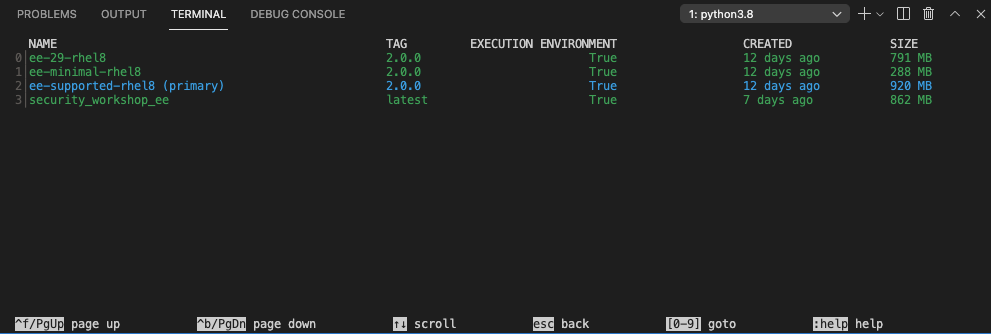
\includegraphics{images/01_navigator-images.png}
\caption{ansible-navigator images}
\end{figure}

\begin{quote}
Note: The output you see might differ from the above output
\end{quote}

This command gives you information about all currently installed
Execution Environments or EEs for short. Investigate an EE by pressing
the corresponding number. For example pressing \textbf{2} with the above
example will open the \texttt{ee-supported-rhel8} execution environment:

\begin{figure}[H]
\centering
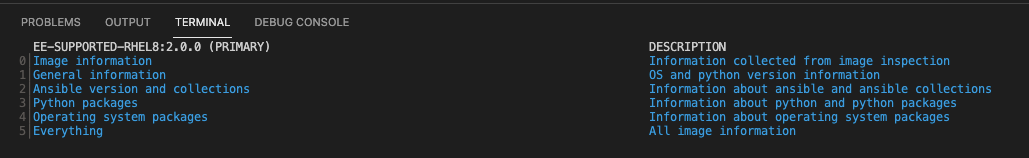
\includegraphics{images/01_navigator-ee-menu.png}
\caption{ee main menu}
\end{figure}

Selecting \texttt{2} for \texttt{Ansible\ version\ and\ collections}
will show us all Ansible Collections installed on that particular EE,
and the version of \texttt{ansible-core}:

\begin{figure}[H]
\centering
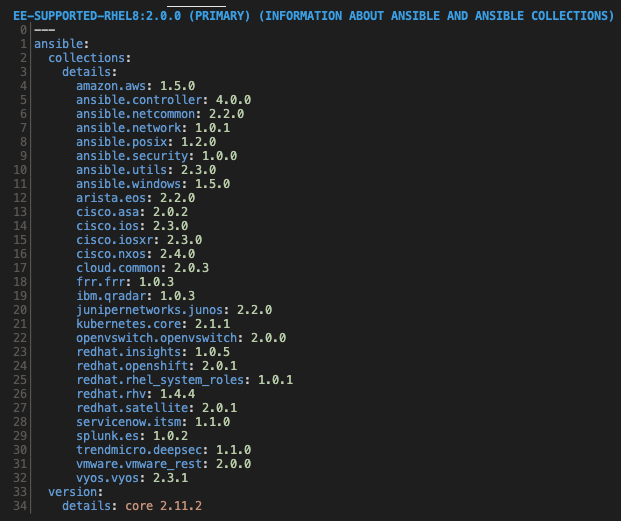
\includegraphics{images/01_navigator-ee-collections.png}
\caption{ee info}
\end{figure}

\hypertarget{step-4---examining-the-ansible-navigator-configuration}{%
\subsubsection{Step 4 - Examining the ansible-navigator
configuration}\label{step-4---examining-the-ansible-navigator-configuration}}

Either use Visual Studio Code to open or use the \texttt{cat} command to
view the contents of the \texttt{ansible-navigator.yml} file. The file
is located in the home directory:

\begin{Shaded}
\begin{Highlighting}[]
\ExtensionTok{$}\NormalTok{ cat \textasciitilde{}/.ansible{-}navigator.yml}
\ExtensionTok{{-}{-}{-}}
\ExtensionTok{ansible{-}navigator:}
  \ExtensionTok{ansible:}
    \ExtensionTok{inventory:}
      \ExtensionTok{entries:}
      \ExtensionTok{{-}}\NormalTok{ \textasciitilde{}/hosts}
  \ExtensionTok{execution{-}environment:}
    \ExtensionTok{image:}\NormalTok{ registry.redhat.io/ansible-automation-platform-24/ee-supported-rhel8:latest}
    \ExtensionTok{enabled:}\NormalTok{ true}
    \ExtensionTok{container{-}engine:}\NormalTok{ podman}
    \ExtensionTok{pull:}
      \ExtensionTok{policy:}\NormalTok{ missing}
    \ExtensionTok{volume{-}mounts:}
    \ExtensionTok{{-}}\NormalTok{ src: }\StringTok{/etc/ansible}
      \ExtensionTok{dest:} \StringTok{/etc/ansible}
\end{Highlighting}
\end{Shaded}

Note the following parameters within the \texttt{.ansible-navigator.yml}
file:

\begin{itemize}
\tightlist
\item
  \texttt{inventories}: shows the location of the ansible inventory
  being used
\item
  \texttt{execution-environment}: where the default execution
  environment is set
\end{itemize}

For a full listing of every configurable knob checkout the
\href{https://ansible.readthedocs.io/projects/navigator/settings/}{documentation}

\hypertarget{step-5---challenge-labs}{%
\subsubsection{Step 5 - Challenge Labs}\label{step-5---challenge-labs}}

You will soon discover that many chapters in this lab guide come with a
``Challenge Lab'' section. These labs are meant to give you a small task
to solve using what you have learned so far. The solution of the task is
shown underneath a warning sign.

\hypertarget{the-ansible-basics}{%
\section{\texorpdfstring{The Ansible Basics
}{The Ansible Basics }}\label{the-ansible-basics}}

\hypertarget{objective}{%
\subsection{Objective}\label{objective}}

In this exercise, we are going to explore the latest Ansible command
line utility \texttt{ansible-navigator} to learn how to work with
inventory files and the listing of modules when needing assistance. The
goal is to familarize yourself with how \texttt{ansible-navigator} works
and how it can be used to enrich your Ansible experience.

This exercise will cover

\begin{itemize}
\tightlist
\item
  Working with inventory files
\item
  Locating and understanding an \texttt{ini} formatted inventory file
\item
  Listing modules and getting help when trying to use them
\end{itemize}

\hypertarget{guide}{%
\subsection{Guide}\label{guide}}

\hypertarget{step-1---work-with-your-inventory}{%
\subsubsection{Step 1 - Work with your
Inventory}\label{step-1---work-with-your-inventory}}

An inventory file is a text file that specifies the nodes that will be
managed by the control machine. The nodes to be managed may include a
list of hostnames or IP addresses of those nodes. The inventory file
allows for nodes to be organized into groups by declaring a host group
name within square brackets ({[}{]}).

To use the \texttt{ansible-navigator} command for host management, you
need to provide an inventory file which defines a list of hosts to be
managed from the control node. In this lab, the inventory is provided by
your instructor. The inventory file is an \texttt{ini} formatted file
listing your hosts, sorted in groups, additionally providing some
variables. It looks like:

\begin{Shaded}
\begin{Highlighting}[]
\ExtensionTok{[web]}
\ExtensionTok{node}\NormalTok{ ansible\_host=}\OperatorTok{\textless{}}\NormalTok{10.3.48.[100+PARTICIPANT_ID]}\OperatorTok{\textgreater{}}

\ExtensionTok{[control]}
\ExtensionTok{controller}\NormalTok{ ansible\_host=10.3.48.100}
\end{Highlighting}
\end{Shaded}

Ansible is already configured to use the inventory specific to your
environment. We will show you in the next step how that is done. For
now, we will execute some simple commands to work with the inventory.

To reference all the inventory hosts, you supply a pattern to the
\texttt{ansible-navigator} command.
\texttt{ansible-navigator\ inventory} has a \texttt{-\/-list} option
which can be useful for displaying all the hosts that are part of an
inventory file including what groups they are associated with.

\begin{Shaded}
\begin{Highlighting}[]
\ExtensionTok{[student@controller}\NormalTok{ rhel\_workshop]$ cd /home/student}
\ExtensionTok{[student@controller}\NormalTok{ \textasciitilde{}]$ ansible{-}navigator inventory }\AttributeTok{{-}{-}list} \AttributeTok{{-}m}\NormalTok{ stdout}
\ExtensionTok{\{}
    \StringTok{"\_meta"}\ExtensionTok{:}\NormalTok{ \{}
        \StringTok{"hostvars"}\ExtensionTok{:}\NormalTok{ \{}
            \StringTok{"controller"}\ExtensionTok{:}\NormalTok{ \{}
                \StringTok{"ansible\_host"}\ExtensionTok{:} \StringTok{"10.3.48.100"}
            \ExtensionTok{\},}
            \StringTok{"node"}\ExtensionTok{:}\NormalTok{ \{}
                \StringTok{"ansible\_host"}\ExtensionTok{:} \StringTok{"10.3.48.101"}
            \ExtensionTok{\}}
        \ExtensionTok{\}}
    \ExtensionTok{\}}\ExtensionTok{,}
    \StringTok{"all"}\ExtensionTok{:}\NormalTok{ \{}
        \StringTok{"children"}\ExtensionTok{:}\NormalTok{ [}
            \StringTok{"control"}\ExtensionTok{,}
            \StringTok{"ungrouped"}\ExtensionTok{,}
            \StringTok{"web"}
        \ExtensionTok{]}
    \ExtensionTok{\}}\ExtensionTok{,}
    \StringTok{"control"}\ExtensionTok{:}\NormalTok{ \{}
        \StringTok{"hosts"}\ExtensionTok{:}\NormalTok{ [}
            \StringTok{"controller"}
        \ExtensionTok{]}
    \ExtensionTok{\}}\ExtensionTok{,}
    \StringTok{"web"}\ExtensionTok{:}\NormalTok{ \{}
        \StringTok{"hosts"}\ExtensionTok{:}\NormalTok{ [}
            \StringTok{"node"}
        \ExtensionTok{]}
    \ExtensionTok{\}}
\ExtensionTok{\}}
\end{Highlighting}
\end{Shaded}

NOTE: \texttt{-m} is short for \texttt{-\/-mode} which allows for the
mode to be switched to standard output instead of using the text-based
user interface (TUI).

If the \texttt{-\/-list} is too verbose, the option of
\texttt{-\/-graph} can be used to provide a more condensed version of
\texttt{-\/-list}.

\begin{Shaded}
\begin{Highlighting}[]
\ExtensionTok{[student@controller}\NormalTok{ \textasciitilde{}]$ ansible{-}navigator inventory }\AttributeTok{{-}{-}graph} \AttributeTok{{-}m}\NormalTok{ stdout}
\ExtensionTok{@all:}
  \KeywordTok{|}\ExtensionTok{{-}{-}@control:}
  \KeywordTok{|}  \KeywordTok{|}\ExtensionTok{{-}{-}controller}
  \KeywordTok{|}\ExtensionTok{{-}{-}@ungrouped:}
  \KeywordTok{|}\ExtensionTok{{-}{-}@web:}
  \KeywordTok{|}  \KeywordTok{|}\ExtensionTok{{-}{-}node}
\end{Highlighting}
\end{Shaded}

We can clearly see that nodes: \texttt{node} is part of the \texttt{web} group, while
\texttt{controller} is part of the \texttt{control} group.

An inventory file can contain a lot more information, it can organize
your hosts in groups or define variables. In our example, the current
inventory has the groups \texttt{web} and \texttt{control}. Run Ansible
with these host patterns and observe the output:

Using the \texttt{ansible-navigator\ inventory} command, we can also run
commands that provide information only for one host or group. For
example, give the following commands a try to see their output.

\begin{Shaded}
\begin{Highlighting}[]
\ExtensionTok{[student@controller}\NormalTok{ \textasciitilde{}]$ ansible{-}navigator inventory }\AttributeTok{{-}{-}graph}\NormalTok{ web }\AttributeTok{{-}m}\NormalTok{ stdout}
\ExtensionTok{[student@controller}\NormalTok{ \textasciitilde{}]$ ansible{-}navigator inventory }\AttributeTok{{-}{-}graph}\NormalTok{ control }\AttributeTok{{-}m}\NormalTok{ stdout}
\ExtensionTok{[student@controller}\NormalTok{ \textasciitilde{}]$ ansible{-}navigator inventory }\AttributeTok{{-}{-}host}\NormalTok{ node }\AttributeTok{{-}m}\NormalTok{ stdout}
\end{Highlighting}
\end{Shaded}

\begin{quote}
\textbf{Tip}

The inventory can contain more data. E.g. if you have hosts that run on
non-standard SSH ports you can put the port number after the hostname
with a colon. Or you could define names specific to Ansible and have
them point to the ``real'' IP or hostname.
\end{quote}

\hypertarget{step-2---listing-modules-and-getting-help}{%
\subsubsection{Step 2 - Listing Modules and Getting
Help}\label{step-2---listing-modules-and-getting-help}}

Ansible Automation Platform comes with multiple supported Execution
Environments (EEs). These EEs come with bundled supported collections
that contain supported content, including modules.

\begin{quote}
\textbf{Tip}

In \texttt{ansible-navigator} exit by pressing the button \texttt{ESC}.
\end{quote}

To browse your available modules first enter interactive mode:

\begin{Shaded}
\begin{Highlighting}[]
\ExtensionTok{$}\NormalTok{ ansible{-}navigator}
\end{Highlighting}
\end{Shaded}

\begin{figure}[H]
\centering
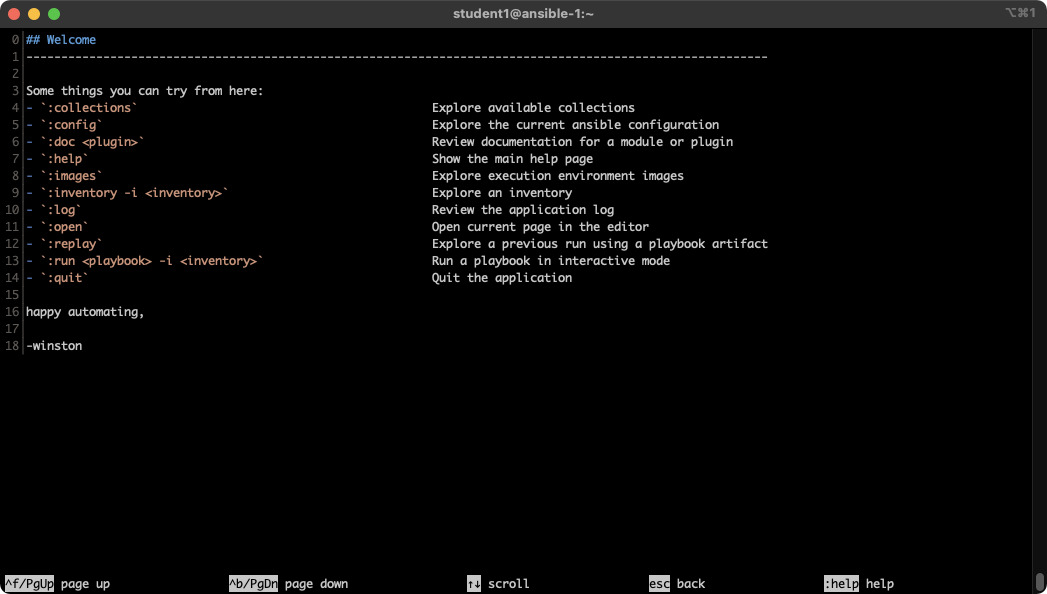
\includegraphics{images/01_interactive-mode.png}
\caption{picture of ansible-navigator}
\end{figure}

First browse a collection by typing \texttt{:collections}

\begin{Shaded}
\begin{Highlighting}[]
\ExtensionTok{:collections}
\end{Highlighting}
\end{Shaded}

\begin{figure}[H]
\centering
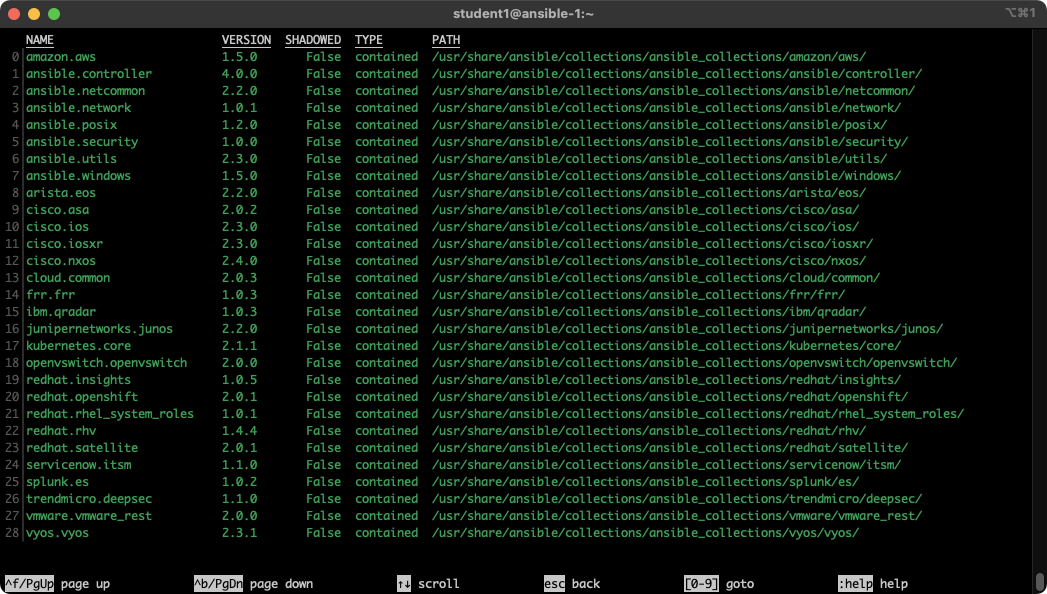
\includegraphics{images/01_interactive-collections.png}
\caption{picture of ansible-navigator}
\end{figure}

To browse the content for a specific collections, type the corresponding
number. For example in the example screenshot above the number
\texttt{0} corresponds to \texttt{amazon.aws} collection. To zoom into
collection type the number \texttt{0}.

\begin{Shaded}
\begin{Highlighting}[]
\ExtensionTok{0}
\end{Highlighting}
\end{Shaded}

\begin{figure}[H]
\centering
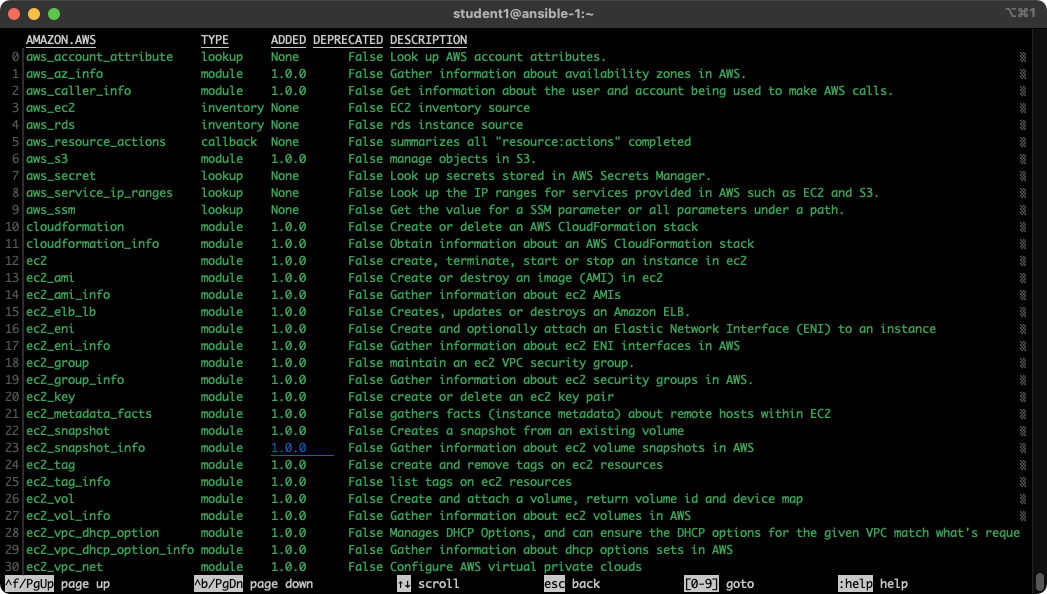
\includegraphics{images/01_interactive-aws.png}
\caption{picture of ansible-navigator}
\end{figure}

Get help for a specific module including usage by zooming in further.
For example the module \texttt{ec2\_metadata\_facts} corresponds to \texttt{3}.

\begin{Shaded}
\begin{Highlighting}[]
\ExtensionTok{:3}
\end{Highlighting}
\end{Shaded}

Scrolling down using the arrow keys or page-up and page-down can show us
documentation and examples.

\begin{figure}[H]
\centering
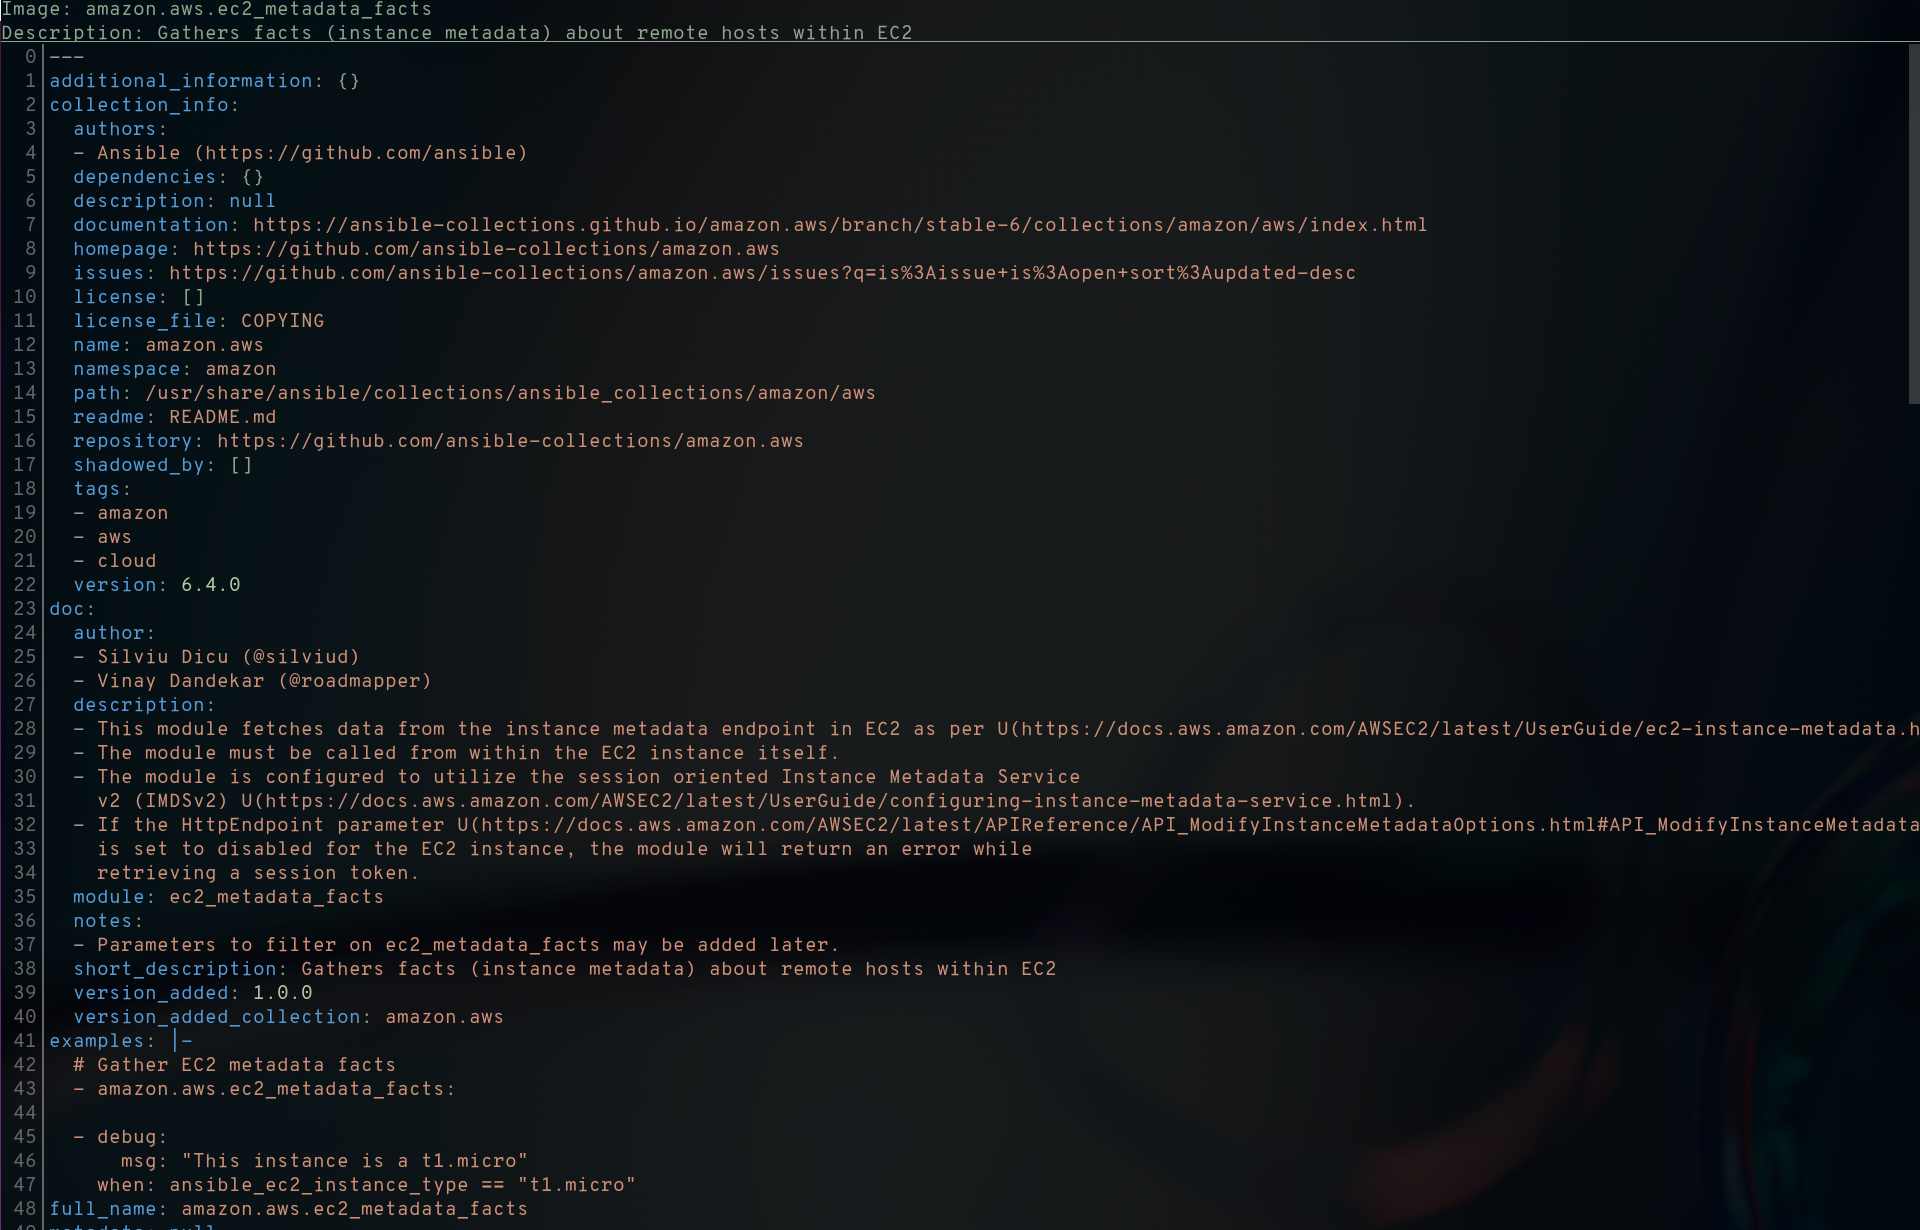
\includegraphics{images/01_interactive-ec2-metadata.png}
\caption{picture of ansible-navigator}
\end{figure}

You can also skip directly to a particular module by simply typing
\texttt{:doc\ namespace.collection.module-name}. For example typing
\texttt{:doc\ amazon.aws.ec2\_metadata\_facts} would skip directly to the final page
shown above.

\begin{quote}
\textbf{Tip}

Different execution environments can have access to different
collections, and different versions of those collections. By using the
built-in documentation you know that it will be accurate for that
particular version of the collection.
\end{quote}

\hypertarget{writing-your-first-playbook}{%
\section{Writing Your First
Playbook}\label{writing-your-first-playbook}}

\hypertarget{objective}{%
\subsection{Objective}\label{objective}}

This exercise covers using Ansible to build an Apache web server on
Red Hat Enterprise Linux. This exercise covers the following Ansible
fundamentals:

\begin{itemize}
\tightlist
\item
  Understanding Ansible module parameters
\item
  Understanding and using the following modules

  \begin{itemize}
  \tightlist
  \item
    \href{https://docs.ansible.com/ansible/latest/modules/dnf_module.html}{dnf
    module}
  \item
    \href{https://docs.ansible.com/ansible/latest/modules/service_module.html}{service
    module}
  \item
    \href{https://docs.ansible.com/ansible/latest/modules/copy_module.html}{copy
    module}
  \end{itemize}
\item
  Understanding
  \href{https://en.wikipedia.org/wiki/Idempotence}{Idempotence} and how
  Ansible modules can be idempotent
\end{itemize}

\hypertarget{guide}{%
\subsection{Guide}\label{guide}}

Playbooks are files which describe the desired configurations or steps
to implement on managed hosts. Playbooks can change lengthy, complex
administrative tasks into easily repeatable routines with predictable
and successful outcomes.

A playbook can have multiple plays and a play can have one or multiple
tasks. In a task a \emph{module} is called, like the modules in the
previous chapter. The goal of a \emph{play} is to map a group of hosts.
The goal of a \emph{task} is to implement modules against those hosts.

\begin{quote}
\textbf{Tip}

Here is a nice analogy: When Ansible modules are the tools in your
workshop, the inventory is the materials and the Playbooks are the
instructions.
\end{quote}

\hypertarget{step-1---playbook-basics}{%
\subsubsection{Step 1 - Playbook
Basics}\label{step-1---playbook-basics}}

Playbooks are text files written in YAML format and therefore need:

\begin{itemize}
\item
  to start with three dashes (\texttt{-\/-\/-})
\item
  proper indentation using spaces and \textbf{not} tabs!
\end{itemize}

There are some important concepts:

\begin{itemize}
\item
  \textbf{hosts}: the managed hosts to perform the tasks on
\item
  \textbf{tasks}: the operations to be performed by invoking Ansible
  modules and passing them the necessary options
\item
  \textbf{become}: privilege escalation in playbooks
\end{itemize}

\begin{quote}
\textbf{Warning}

The ordering of the contents within a Playbook is important, because
Ansible executes plays and tasks in the order they are presented.
\end{quote}

A Playbook should be \textbf{idempotent}, so if a Playbook is run once
to put the hosts in the correct state, it should be safe to run it a
second time and it should make no further changes to the hosts.

\begin{quote}
\textbf{Tip}

Most Ansible modules are idempotent, so it is relatively easy to ensure
this is true.
\end{quote}

\hypertarget{step-2---creating-a-directory-structure-and-file-for-your-playbook}{%
\subsubsection{Step 2 - Creating a Directory Structure and File for your
Playbook}\label{step-2---creating-a-directory-structure-and-file-for-your-playbook}}

Enough theory, it's time to create your first Ansible playbook. In this
lab you create a playbook to set up an Apache web server in three steps:

\begin{enumerate}
\def\labelenumi{\arabic{enumi}.}
\tightlist
\item
  Install httpd package
\item
  Enable/start httpd service
\item
  Copy over an web.html file to each web host
\end{enumerate}

This Playbook makes sure the package containing the Apache web server is
installed on \texttt{node}.

There is a
\href{https://docs.ansible.com/ansible/latest/user_guide/playbooks_best_practices.html}{best
practice} on the preferred directory structures for playbooks. We
strongly encourage you to read and understand these practices as you
develop your Ansible ninja skills. That said, our playbook today is very
basic and creating a complex structure will just confuse things.

Instead, we are going to create a very simple directory structure for
our playbook, and add just a couple of files to it.

On your control host \textbf{ansible}, create a directory called
\texttt{ansible-files} in your home directory and change directories
into it:

\begin{Shaded}
\begin{Highlighting}[]
\ExtensionTok{[student@controller}\NormalTok{ \textasciitilde{}]$ mkdir ansible{-}files}
\ExtensionTok{[student@controller}\NormalTok{ \textasciitilde{}]$ cd ansible{-}files/}
\end{Highlighting}
\end{Shaded}

Add a file called \texttt{apache.yml} with the following content. As
discussed in the previous exercises, use \texttt{vi}/\texttt{vim} or \texttt{nano}.

\begin{Shaded}
\begin{Highlighting}[]
\PreprocessorTok{{-}{-}{-}}
\KeywordTok{{-}}\AttributeTok{ }\FunctionTok{name}\KeywordTok{:}\AttributeTok{ Apache server installed}
\AttributeTok{  }\FunctionTok{hosts}\KeywordTok{:}\AttributeTok{ node}
\AttributeTok{  }\FunctionTok{become}\KeywordTok{:}\AttributeTok{ }\CharTok{True}
\end{Highlighting}
\end{Shaded}

This shows one of Ansible's strengths: The Playbook syntax is easy to
read and understand. In this Playbook:

\begin{itemize}
\tightlist
\item
  A name is given for the play via \texttt{name:}.
\item
  The host to run the playbook against is defined via \texttt{hosts:}.
\item
  We enable user privilege escalation with \texttt{become:}.
\end{itemize}

\begin{quote}
\textbf{Tip}

You obviously need to use privilege escalation to install a package or
run any other task that requires root permissions. This is done in the
Playbook by \texttt{become:\ yes}.
\end{quote}

Now that we've defined the play, let's add a task to get something done.
We will add a task in which dnf will ensure that the Apache package is
installed in the latest version. Modify the file so that it looks like
the following listing:

\begin{Shaded}
\begin{Highlighting}[]
\PreprocessorTok{{-}{-}{-}}
\KeywordTok{{-}}\AttributeTok{ }\FunctionTok{name}\KeywordTok{:}\AttributeTok{ Apache server installed}
\AttributeTok{  }\FunctionTok{hosts}\KeywordTok{:}\AttributeTok{ node}
\AttributeTok{  }\FunctionTok{become}\KeywordTok{:}\AttributeTok{ }\CharTok{True}
\AttributeTok{  }\FunctionTok{tasks}\KeywordTok{:}
\AttributeTok{    }\KeywordTok{{-}}\AttributeTok{ }\FunctionTok{name}\KeywordTok{:}\AttributeTok{ Install Apache}
\AttributeTok{      }\FunctionTok{ansible.builtin.dnf}\KeywordTok{:}
\AttributeTok{        }\FunctionTok{name}\KeywordTok{:}\AttributeTok{ httpd}
\end{Highlighting}
\end{Shaded}

\begin{quote}
\textbf{Tip}

Since playbooks are written in YAML, alignment of the lines and keywords
is crucial. Make sure to vertically align the \emph{t} in \texttt{task}
with the \emph{b} in \texttt{become}. Once you are more familiar with
Ansible, make sure to take some time and study a bit the
\href{https://docs.ansible.com/ansible/latest/reference_appendices/YAMLSyntax.html}{YAML
Syntax}.
\end{quote}

In the added lines:

\begin{itemize}
\tightlist
\item
  We started the tasks part with the keyword \texttt{tasks:}.
\item
  A task is named and the module for the task is referenced. Here it
  uses the \texttt{dnf} module.
\item
  Parameters for the module are added:

  \begin{itemize}
  \tightlist
  \item
    \texttt{name:} to identify the package name
  \item
    \texttt{state:} to define the wanted state of the package
  \end{itemize}
\end{itemize}

\begin{quote}
\textbf{Tip}

The module parameters are individual to each module. If in doubt, look
them up again with \texttt{ansible-doc}.
\end{quote}

Save your playbook and exit your editor.

\hypertarget{step-3---running-the-playbook}{%
\subsubsection{Step 3 - Running the
Playbook}\label{step-3---running-the-playbook}}

With the introduction of Ansible Automation Platform 2, several new key
components are being introduced as a part of the overall developer
experience. Execution environments have been introduced to provide
predictable environments to be used during automation runtime. All
collection dependencies are contained within the execution environment
to ensure that automation created in development environments runs the
same as in production environments.

What do you find within an execution environment?

\begin{itemize}
\tightlist
\item
  RHEL UBI 8
\item
  Ansible 2.9 or Ansible Core 2.11
\item
  Python 3.8
\item
  Any content Collections
\item
  Collection python or binary dependencies.
\end{itemize}

Why use execution environments?

They provide a standardized way to define, build and distribute the
environments that the automation runs in. In a nutshell, Automation
execution environments are container images that allow for easier
administration of Ansible by the platform administrator.

Considering the shift towards containerized execution of automation,
automation development workflow and tooling that existed before Ansible
Automation Platform 2 have had to be reimagined. In short,
\texttt{ansible-navigator} replaces \texttt{ansible-playbook} and other
\texttt{ansible-*} command line utilities.

With this change, Ansible playbooks are executed using the
\texttt{ansible-navigator} command on the control node.

The prerequisites and best practices for using
\texttt{ansible-navigator} have been done for you within this lab.

These include:
\begin{itemize}
\tightlist
\item Installing the \texttt{ansible-navigator} package
\item Creating a default settings \texttt{\textasciitilde{}/.ansible-navigator.yml} for all your projects (optional)
\item All execution environment (EE) logs are stored within the execution folder
\end{itemize}

For more information on the
\href{https://github.com/ansible/ansible-navigator/blob/main/docs/settings.rst}{Ansible
navigator settings}

\begin{quote}
\textbf{Tip}

The parameters for ansible-navigator maybe modified for your specific
environment. The current settings use a default
\texttt{ansible-navigator.yml} for all projects, but a specific
\texttt{ansible-navigator.yml} can be created for each project and is
the recommended practice.
\end{quote}

To run your playbook, use the
\texttt{ansible-navigator\ run\ \textless{}playbook\textgreater{}}
command as follows:

\begin{Shaded}
\begin{Highlighting}[]
\ExtensionTok{[student@controller}\NormalTok{ ansible{-}files]$ ansible{-}navigator run apache.yml}
\end{Highlighting}
\end{Shaded}

\begin{quote}
\textbf{Tip}

The existing \texttt{ansible-navigator.yml} file provides the location
of your inventory file. If this was not set within your
\texttt{ansible-navigator.yml} file, the command to run the playbook
would be:
\texttt{ansible-navigator\ run\ apache.yml\ -i\ \textasciitilde{}/hosts}
\end{quote}

When running the playbook, you'll be displayed a text user interface
(TUI) that displays the play name among other information about the
playbook that is currently run.

\begin{Shaded}
\begin{Highlighting}[]
  \ExtensionTok{PLAY}\NormalTok{ NAME                        OK  CHANGED    UNREACHABLE      FAILED    SKIPPED    IGNORED    IN PROGRESS     TASK COUNT          PROGRESS}
\ExtensionTok{0│Apache}\NormalTok{ server installed           2        1              0           0          0          0              0              2          COMPLETE}
\end{Highlighting}
\end{Shaded}

If you notice, prior to the play name
\texttt{Apache\ server\ installed}, you'll see a \texttt{0}. By pressing
the \texttt{0} key on your keyboard, you will be provided a new window
view displaying the different tasks that ran for the playbook
completion. In this example, those tasks included the ``Gathering
Facts'' and ``Install Apache''. The ``Gathering Facts'' is a built-in
task that runs automatically at the beginning of each play. It collects
information about the managed nodes. Exercises later on will cover this
in more detail. The ``Install Apache'' was the task created within the
\texttt{apache.yml} file that installed \texttt{httpd}.

The display should look something like this:

\begin{Shaded}
\begin{Highlighting}[]
  \ExtensionTok{RESULT}\NormalTok{      HOST  NUMBER      CHANGED       TASK                                                   TASK ACTION           DURATION}
\ExtensionTok{0│OK}\NormalTok{          node          0        False       Gathering Facts                                        gather\_facts                1s}
\ExtensionTok{1│OK}\NormalTok{          node          1         True       Install Apache                        dnf                         4s}
\end{Highlighting}
\end{Shaded}

Taking a closer look, you'll notice that each task is associated with a
number. Task 1, ``Install Apache'', had a change and used the
\texttt{dnf} module. In this case, the change is the installation of
Apache (\texttt{httpd} package) on the host \texttt{node}.

By pressing \texttt{0} or \texttt{1} on your keyboard, you can see
further details of the task being run. If a more traditional output view
is desired, type \texttt{:st} within the text user interface.

Once you've completed, reviewing your Ansible playbook, you can exit out
of the TUI via the Esc key on your keyboard.

\begin{quote}
\textbf{Tip}

The Esc key only takes you back to the previous screen. Once at the main
overview screen an additional Esc key will take you back to the terminal
window.
\end{quote}

Once the playbook has completed, connect to \texttt{node} via SSH to
make sure Apache has been installed:

\begin{Shaded}
\begin{Highlighting}[]
\ExtensionTok{[student@controller}\NormalTok{ ansible{-}files]$ ssh root@10.3.48.[100+PARTICIPANT\_ID]}
\ExtensionTok{Last}\NormalTok{ login: Thu Jan 11 10:35:34 2024 from 10.3.48.100}
\end{Highlighting}
\end{Shaded}

Use the command \texttt{rpm\ -qi\ httpd} to verify httpd is installed:

\begin{Shaded}
\begin{Highlighting}[]
\ExtensionTok{[ec2{-}user@node}\NormalTok{ \textasciitilde{}]$ rpm }\AttributeTok{{-}qi}\NormalTok{ httpd}
\ExtensionTok{Name}\NormalTok{        : httpd}
\ExtensionTok{Version}\NormalTok{     : 2.4.37}
\ExtensionTok{[...]}
\end{Highlighting}
\end{Shaded}

Log out of \texttt{node} with the command \texttt{exit} so that you are
back on the control host and verify the installed package with an
Ansible playbook labeled \texttt{package.yml}

\begin{Shaded}
\begin{Highlighting}[]
\PreprocessorTok{{-}{-}{-}}
\KeywordTok{{-}}\AttributeTok{ }\FunctionTok{name}\KeywordTok{:}\AttributeTok{ Check packages}
\AttributeTok{  }\FunctionTok{hosts}\KeywordTok{:}\AttributeTok{ node}
\AttributeTok{  }\FunctionTok{become}\KeywordTok{:}\AttributeTok{ }\CharTok{True}
\AttributeTok{  }\FunctionTok{vars}\KeywordTok{:}
\AttributeTok{    }\FunctionTok{p}\KeywordTok{:}\AttributeTok{ httpd}
\AttributeTok{  }\FunctionTok{tasks}\KeywordTok{:}
\AttributeTok{    }\KeywordTok{{-}}\AttributeTok{ }\FunctionTok{name}\KeywordTok{:}\AttributeTok{ Gather the packages facts}
\AttributeTok{      }\FunctionTok{ansible.builtin.package\_facts}\KeywordTok{:}
\AttributeTok{        }\FunctionTok{manager}\KeywordTok{:}\AttributeTok{ auto}
\AttributeTok{    }\KeywordTok{{-}}\AttributeTok{ }\FunctionTok{name}\KeywordTok{:}\StringTok{ "Check whether \{\{ p \}\} is installed"}
\AttributeTok{      }\FunctionTok{ansible.builtin.debug}\KeywordTok{:}
\AttributeTok{        }\FunctionTok{msg}\KeywordTok{:}\AttributeTok{ }\StringTok{"\{\{ p \}\} \{\{ ansible\_facts.packages[p][0].version \}\} is installed!"}
\AttributeTok{      }\FunctionTok{when}\KeywordTok{:}\AttributeTok{ p in ansible\_facts.packages}
\end{Highlighting}
\end{Shaded}

You can now run it similarly to the previous one:

\begin{Shaded}
\begin{Highlighting}[]
\ExtensionTok{[student@controller}\NormalTok{ \textasciitilde{}]$ ansible{-}navigator run package.yml }\AttributeTok{{-}m}\NormalTok{ stdout}
\end{Highlighting}
\end{Shaded}

\begin{Shaded}
\begin{Highlighting}[]

\ExtensionTok{PLAY}\NormalTok{ [Check packages] }\PreprocessorTok{**********************************************************}

\ExtensionTok{TASK}\NormalTok{ [Gathering Facts] }\PreprocessorTok{*********************************************************}
\ExtensionTok{ok:} \PreprocessorTok{[}\SpecialStringTok{ansible}\PreprocessorTok{]}

\ExtensionTok{TASK}\NormalTok{ [Gather the packages facts] }\PreprocessorTok{************************************************}
\ExtensionTok{ok:} \PreprocessorTok{[}\SpecialStringTok{ansible}\PreprocessorTok{]}

\ExtensionTok{TASK}\NormalTok{ [Check whether httpd is installed] }\PreprocessorTok{*************************************}
\ExtensionTok{ok:} \PreprocessorTok{[}\SpecialStringTok{ansible}\PreprocessorTok{]}\NormalTok{ =}\OperatorTok{\textgreater{}}\NormalTok{ \{}
    \StringTok{"msg"}\ExtensionTok{:} \StringTok{"httpd 2.4.37 is installed!"}
\NormalTok{\}}

\ExtensionTok{PLAY}\NormalTok{ RECAP }\PreprocessorTok{*********************************************************************}
\ExtensionTok{ansible}\NormalTok{: ok=3  changed=0  unreachable=0  failed=0  skipped=0  rescued=0  ignored=0}
\end{Highlighting}
\end{Shaded}

Run the the \texttt{ansible-navigator\ run\ apache.yml} playbook for a
second time, and compare the output. The output ``CHANGED'' now shows
\texttt{0} instead of \texttt{1} and the color changed from yellow to
green. This makes it easier to spot when changes have occured when
running the Ansible playbook.

\hypertarget{step-4---extend-your-playbook-start-enable-apache}{%
\subsubsection{Step 4 - Extend your Playbook: Start \& Enable
Apache}\label{step-4---extend-your-playbook-start-enable-apache}}

The next part of the Ansible playbook makes sure the Apache application
is enabled and started on \texttt{node}.

On the control host, as your student user, edit the file
\texttt{\textasciitilde{}/ansible-files/apache.yml} to add a second task
using the \texttt{service} module. The Playbook should now look like
this:

\begin{Shaded}
\begin{Highlighting}[]
\PreprocessorTok{{-}{-}{-}}
\KeywordTok{{-}}\AttributeTok{ }\FunctionTok{name}\KeywordTok{:}\AttributeTok{ Apache server installed}
\AttributeTok{  }\FunctionTok{hosts}\KeywordTok{:}\AttributeTok{ node}
\AttributeTok{  }\FunctionTok{become}\KeywordTok{:}\AttributeTok{ }\CharTok{True}
\AttributeTok{  }\FunctionTok{tasks}\KeywordTok{:}
\AttributeTok{    }\KeywordTok{{-}}\AttributeTok{ }\FunctionTok{name}\KeywordTok{:}\AttributeTok{ Install Apache}
\AttributeTok{      }\FunctionTok{ansible.builtin.dnf}\KeywordTok{:}
\AttributeTok{        }\FunctionTok{name}\KeywordTok{:}\AttributeTok{ httpd}
\AttributeTok{    }\KeywordTok{{-}}\AttributeTok{ }\FunctionTok{name}\KeywordTok{:}\AttributeTok{ Apache enabled and running}
\AttributeTok{      }\FunctionTok{ansible.builtin.service}\KeywordTok{:}
\AttributeTok{        }\FunctionTok{name}\KeywordTok{:}\AttributeTok{ httpd}
\AttributeTok{        }\FunctionTok{enabled}\KeywordTok{:}\AttributeTok{ }\CharTok{True}
\AttributeTok{        }\FunctionTok{state}\KeywordTok{:}\AttributeTok{ started}
\end{Highlighting}
\end{Shaded}

What exactly did we do?

\begin{itemize}
\tightlist
\item
  a second task named ``Apache enabled and running'' is created
\item
  a module is specified (\texttt{service})
\item
  The module \texttt{service} takes the name of the service
  (\texttt{httpd}), if it should be permanently set (\texttt{enabled}),
  and its current state (\texttt{started})
\end{itemize}

Thus with the second task we make sure the Apache server is indeed
running on the target machine. Run your extended Playbook:

\begin{Shaded}
\begin{Highlighting}[]
\ExtensionTok{[student@controller}\NormalTok{ \textasciitilde{}]$ ansible{-}navigator run apache.yml}
\end{Highlighting}
\end{Shaded}

Notice in the output, we see the play had \texttt{1} ``CHANGED'' shown
in yellow and if we press \texttt{0} to enter the play output, you can
see that task 2, ``Apache enabled and running'', was the task that
incorporated the latest change by the ``CHANGED'' value being set to
True and highlighted in yellow.

\begin{itemize}
\item
  Run the playbook a second time using \texttt{ansible-navigator} to get
  used to the change in the output.
\item
  Use an Ansible playbook labeled \texttt{service\_state.yml} to make sure the
  Apache (httpd) service is running on \texttt{node}, e.g.~with:
  \texttt{systemctl\ status\ httpd}.
\end{itemize}

\begin{Shaded}
\begin{Highlighting}[]
\PreprocessorTok{{-}{-}{-}}
\KeywordTok{{-}}\AttributeTok{ }\FunctionTok{name}\KeywordTok{:}\AttributeTok{ Check Status}
\AttributeTok{  }\FunctionTok{hosts}\KeywordTok{:}\AttributeTok{ node}
\AttributeTok{  }\FunctionTok{become}\KeywordTok{:}\AttributeTok{ }\CharTok{True}
\AttributeTok{  }\FunctionTok{vars}\KeywordTok{:}
\AttributeTok{    }\FunctionTok{package}\KeywordTok{:}\AttributeTok{ httpd}
\AttributeTok{  }\FunctionTok{tasks}\KeywordTok{:}
\AttributeTok{    }\KeywordTok{{-}}\AttributeTok{ }\FunctionTok{name}\KeywordTok{:}\StringTok{ "Check status of \{\{ package \}\} service"}
\AttributeTok{      }\FunctionTok{ansible.builtin.service\_facts}\KeywordTok{:}
\AttributeTok{      }\FunctionTok{register}\KeywordTok{:}\AttributeTok{ service\_state}
\AttributeTok{    }\KeywordTok{{-}}\AttributeTok{ }\FunctionTok{ansible.builtin.debug}\KeywordTok{:}
\AttributeTok{        }\FunctionTok{var}\KeywordTok{:}\AttributeTok{ service\_state.ansible\_facts.services["\{\{ package \}\}.service"].state}
\end{Highlighting}
\end{Shaded}

\begin{Shaded}
\begin{Highlighting}[]
\ExtensionTok{[student@controller}\NormalTok{ \textasciitilde{}]$ ansible{-}navigator run service\_state.yml}
\end{Highlighting}
\end{Shaded}

\hypertarget{step-5---extend-your-playbook-create-an-web.html}{%
\subsubsection{Step 5 - Extend your Playbook: Create an
web.html}\label{step-5---extend-your-playbook-create-an-web.html}}

Check that the tasks were executed correctly and Apache is accepting
connections: Make an HTTP request using Ansible's \texttt{uri} module in
a playbook named \texttt{check\_httpd.yml} from the control node to
\texttt{node}.

\begin{Shaded}
\begin{Highlighting}[]
\PreprocessorTok{{-}{-}{-}}
\KeywordTok{{-}}\AttributeTok{ }\FunctionTok{name}\KeywordTok{:}\AttributeTok{ Check URL}
\AttributeTok{  }\FunctionTok{hosts}\KeywordTok{:}\AttributeTok{ control}
\AttributeTok{  }\FunctionTok{vars}\KeywordTok{:}
\AttributeTok{    }\FunctionTok{node}\KeywordTok{:}\AttributeTok{ }\StringTok{"[YOUR NODE IP ADDRESS]"}
\AttributeTok{  }\FunctionTok{tasks}\KeywordTok{:}
\AttributeTok{    }\KeywordTok{{-}}\AttributeTok{ }\FunctionTok{name}\KeywordTok{:}\AttributeTok{ Check that you can connect (GET) to a page and it returns a status 200}
\AttributeTok{      }\FunctionTok{ansible.builtin.uri}\KeywordTok{:}
\AttributeTok{        }\FunctionTok{url}\KeywordTok{:}\AttributeTok{ }\StringTok{"http://\{\{ node \}\}"}
\end{Highlighting}
\end{Shaded}

\begin{quote}
\textbf{Warning: Expect a lot of red lines!}
\end{quote}

\begin{Shaded}
\begin{Highlighting}[]
\ExtensionTok{[student@controller}\NormalTok{ \textasciitilde{}]$ ansible{-}navigator run check\_httpd.yml }\AttributeTok{{-}m}\NormalTok{ stdout}
\end{Highlighting}
\end{Shaded}

There are a lot of red lines and an error: As long as there is not at
least an \texttt{web.html} file to be served by Apache, it will throw an
ugly ``HTTP Error 403: Forbidden'' status and Ansible will report an
error.
Also, you are not even seeing the 403 error, since the \texttt{node} port 80 is not reachable due to firewalld's configuration which does not allow connections to be allowed.

Let's start fixing this last issue. To do so, we'll alter the \texttt{apache.yml} file in the following way:

\begin{Shaded}
\begin{Highlighting}[]
\PreprocessorTok{{-}{-}{-}}
\KeywordTok{{-}}\AttributeTok{ }\FunctionTok{name}\KeywordTok{:}\AttributeTok{ Apache server installed}
\AttributeTok{  }\FunctionTok{hosts}\KeywordTok{:}\AttributeTok{ node}
\AttributeTok{  }\FunctionTok{become}\KeywordTok{:}\AttributeTok{ }\CharTok{True}
\AttributeTok{  }\FunctionTok{tasks}\KeywordTok{:}
\AttributeTok{    }\KeywordTok{{-}}\AttributeTok{ }\FunctionTok{name}\KeywordTok{:}\AttributeTok{ Install Apache}
\AttributeTok{      }\FunctionTok{ansible.builtin.dnf}\KeywordTok{:}
\AttributeTok{        }\FunctionTok{name}\KeywordTok{:}\AttributeTok{ httpd}
\AttributeTok{    }\KeywordTok{{-}}\AttributeTok{ }\FunctionTok{name}\KeywordTok{:}\AttributeTok{ Apache enabled and running}
\AttributeTok{      }\FunctionTok{ansible.builtin.service}\KeywordTok{:}
\AttributeTok{        }\FunctionTok{name}\KeywordTok{:}\AttributeTok{ httpd}
\AttributeTok{        }\FunctionTok{enabled}\KeywordTok{:}\AttributeTok{ }\CharTok{True}
\AttributeTok{        }\FunctionTok{state}\KeywordTok{:}\AttributeTok{ started}
\AttributeTok{    }\KeywordTok{{-}}\AttributeTok{ }\FunctionTok{name}\KeywordTok{:}\AttributeTok{ Open firewall port}
\AttributeTok{      }\FunctionTok{ansible.posix.firewalld}\KeywordTok{:}
\AttributeTok{        }\FunctionTok{service}\KeywordTok{:}\AttributeTok{ http}
\AttributeTok{        }\FunctionTok{immediate}\KeywordTok{:}\CharTok{ True}
\AttributeTok{        }\FunctionTok{permanent}\KeywordTok{:}\CharTok{ True}
\AttributeTok{        }\FunctionTok{state}\KeywordTok{:}\AttributeTok{ enabled}
\end{Highlighting}
\end{Shaded}

What does this new task do? The new task uses the \texttt{firewalld}
module and defines the service option (\texttt{HTTP} standard port is \texttt{80/tcp}) and the state enabled.
Due to how the \texttt{firewalld} utility works, we need to tell Ansible that we want the new port to be immediately available and configured in the same way even after reboot (with the \texttt{permanent} option).

Run your extended Playbook:

\begin{Shaded}
\begin{Highlighting}[]
\ExtensionTok{[student@controller}\NormalTok{ ansible{-}files]$ ansible{-}navigator run apache.yml }\AttributeTok{{-}m}\NormalTok{ stdout}
\end{Highlighting}
\end{Shaded}

Now that we have opened the port, you can re-run the \texttt{check\_httpd.yml} playbook and see that we now get the 403 error.

So why not use Ansible to deploy a simple \texttt{web.html} file? On the
ansible control host, as the \texttt{student} user, create the directory
\texttt{files} to hold file resources in
\texttt{\textasciitilde{}/ansible-files/}:

\begin{Shaded}
\begin{Highlighting}[]
\ExtensionTok{[student@controller}\NormalTok{ ansible{-}files]$ mkdir files}
\end{Highlighting}
\end{Shaded}

Then create the file
\texttt{\textasciitilde{}/ansible-files/files/web.html} on the control
node:

\begin{Shaded}
\begin{Highlighting}[]
\DataTypeTok{\textless{}}\KeywordTok{body}\DataTypeTok{\textgreater{}}
\DataTypeTok{  \textless{}}\KeywordTok{h1}\DataTypeTok{\textgreater{}}\NormalTok{Apache is running fine}\DataTypeTok{\textless{}/}\KeywordTok{h1}\DataTypeTok{\textgreater{}}
\DataTypeTok{\textless{}/}\KeywordTok{body}\DataTypeTok{\textgreater{}}
\end{Highlighting}
\end{Shaded}

In a previous example, you used Ansible's \texttt{copy} module to write
text supplied on the command line into a file. Now you'll use the module
in your playbook to copy a file.

On the control node as your student user edit the file
\texttt{\textasciitilde{}/ansible-files/apache.yml} and add a new task
utilizing the \texttt{copy} module. It should now look like this:

\begin{Shaded}
\begin{Highlighting}[]
\PreprocessorTok{{-}{-}{-}}
\KeywordTok{{-}}\AttributeTok{ }\FunctionTok{name}\KeywordTok{:}\AttributeTok{ Apache server installed}
\AttributeTok{  }\FunctionTok{hosts}\KeywordTok{:}\AttributeTok{ node}
\AttributeTok{  }\FunctionTok{become}\KeywordTok{:}\AttributeTok{ }\CharTok{True}
\AttributeTok{  }\FunctionTok{tasks}\KeywordTok{:}
\AttributeTok{    }\KeywordTok{{-}}\AttributeTok{ }\FunctionTok{name}\KeywordTok{:}\AttributeTok{ Install Apache}
\AttributeTok{      }\FunctionTok{ansible.builtin.dnf}\KeywordTok{:}
\AttributeTok{        }\FunctionTok{name}\KeywordTok{:}\AttributeTok{ httpd}
\AttributeTok{    }\KeywordTok{{-}}\AttributeTok{ }\FunctionTok{name}\KeywordTok{:}\AttributeTok{ Apache enabled and running}
\AttributeTok{      }\FunctionTok{ansible.builtin.service}\KeywordTok{:}
\AttributeTok{        }\FunctionTok{name}\KeywordTok{:}\AttributeTok{ httpd}
\AttributeTok{        }\FunctionTok{enabled}\KeywordTok{:}\AttributeTok{ }\CharTok{True}
\AttributeTok{        }\FunctionTok{state}\KeywordTok{:}\AttributeTok{ started}
\AttributeTok{    }\KeywordTok{{-}}\AttributeTok{ }\FunctionTok{name}\KeywordTok{:}\AttributeTok{ Open firewall port}
\AttributeTok{      }\FunctionTok{ansible.posix.firewalld}\KeywordTok{:}
\AttributeTok{        }\FunctionTok{service}\KeywordTok{:}\AttributeTok{ http}
\AttributeTok{        }\FunctionTok{immediate}\KeywordTok{:}\CharTok{ True}
\AttributeTok{        }\FunctionTok{permanent}\KeywordTok{:}\CharTok{ True}
\AttributeTok{        }\FunctionTok{state}\KeywordTok{:}\AttributeTok{ enabled}
\AttributeTok{    }\KeywordTok{{-}}\AttributeTok{ }\FunctionTok{name}\KeywordTok{:}\AttributeTok{ Copy index.html}
\AttributeTok{      }\FunctionTok{ansible.builtin.copy}\KeywordTok{:}
\AttributeTok{        }\FunctionTok{src}\KeywordTok{:}\AttributeTok{ web.html}
\AttributeTok{        }\FunctionTok{dest}\KeywordTok{:}\AttributeTok{ /var/www/html/index.html}
\AttributeTok{        }\FunctionTok{mode}\KeywordTok{:}\AttributeTok{ }\StringTok{\textquotesingle{}644\textquotesingle{}}
\end{Highlighting}
\end{Shaded}

What does this new copy task do? The new task uses the \texttt{copy}
module and defines the source and destination options for the copy
operation as parameters.

Run your extended Playbook:

\begin{Shaded}
\begin{Highlighting}[]
\ExtensionTok{[student@controller}\NormalTok{ ansible{-}files]$ ansible{-}navigator run apache.yml }\AttributeTok{{-}m}\NormalTok{ stdout}
\end{Highlighting}
\end{Shaded}

\begin{itemize}
\item
  Have a good look at the output, notice the changes of ``CHANGED'' and
  the tasks associated with that change.
\item
  Run the Ansible playbook \texttt{check\_httpd.yml} using the \texttt{uri} module
  from above again to test Apache. The command should now return a
  friendly green ``status: 200'' line, amongst other information.
\end{itemize}

\hypertarget{using-variables}{%
\section{Using Variables}\label{using-variables}}

\hypertarget{objective}{%
\subsection{Objective}\label{objective}}

Ansible supports variables to store values that can be used in Ansible
playbooks. Variables can be defined in a variety of places and have a
clear precedence. Ansible substitutes the variable with its value when a
task is executed.

This exercise covers variables, specifically

\begin{itemize}
\tightlist
\item
  How to use variable delimiters \texttt{\{\{} and \texttt{\}\}}
\item
  What \texttt{host\_vars} and \texttt{group\_vars} are and when to use
  them
\item
  How to use \texttt{ansible\_facts}
\item
  How to use the \texttt{debug} module to print variables to the console
  window
\end{itemize}

\hypertarget{guide}{%
\subsection{Guide}\label{guide}}

\hypertarget{intro-to-variables}{%
\subsubsection{Intro to Variables}\label{intro-to-variables}}

Variables are referenced in Ansible Playbooks by placing the variable
name in double curly braces:

\begin{Shaded}
\begin{Highlighting}[]
\AttributeTok{Here comes a variable \{\{ variable1 \}\}}
\end{Highlighting}
\end{Shaded}

Variables and their values can be defined in various places: the
inventory, additional files, on the command line, etc.

The recommended practice to provide variables in the inventory is to
define them in files located in two directories named
\texttt{host\_vars} and \texttt{group\_vars}:

\begin{itemize}
\tightlist
\item
  To define variables for a group ``servers'', a YAML file named
  \texttt{group\_vars/servers.yml} with the variable definitions is
  created.
\item
  To define variables specifically for a host \texttt{node}, the file
  \texttt{host\_vars/node.yml} with the variable definitions is
  created.
\end{itemize}

\begin{quote}
\textbf{Tip}

Host variables take precedence over group variables (more about
precedence can be found in the
\href{https://docs.ansible.com/ansible/latest/user_guide/playbooks_variables.html\#variable-precedence-where-should-i-put-a-variable}{docs}).
\end{quote}

\hypertarget{step-1---create-variable-files}{%
\subsubsection{Step 1 - Create Variable
Files}\label{step-1---create-variable-files}}

For understanding and practice let's do a lab. Following up on the theme
``Let's build a web server. Or two. Or even more\ldots\hspace{0pt}'',
you will change the \texttt{index.html} to show the development
environment (dev/prod) a server is deployed in.

On the ansible control host, as the \texttt{student} user, create the
directories to hold the variable definitions in
\texttt{\textasciitilde{}/ansible-files/}:

\begin{Shaded}
\begin{Highlighting}[]
\ExtensionTok{[student@controller}\NormalTok{ ansible{-}files]$ mkdir host\_vars group\_vars}
\end{Highlighting}
\end{Shaded}

Now create two files containing variable definitions. We'll define a
variable named \texttt{stage} which will point to different
environments, \texttt{dev} or \texttt{prod}:

\begin{itemize}
\tightlist
\item
  Create the file
  \texttt{\textasciitilde{}/ansible-files/group\_vars/web.yml} with this
  content:
\end{itemize}

\begin{Shaded}
\begin{Highlighting}[]
\PreprocessorTok{{-}{-}{-}}
\FunctionTok{stage}\KeywordTok{:}\AttributeTok{ dev}
\end{Highlighting}
\end{Shaded}

\begin{itemize}
\tightlist
\item
  Create the file
  \texttt{\textasciitilde{}/ansible-files/host\_vars/node.yml} with
  this content:
\end{itemize}

\begin{Shaded}
\begin{Highlighting}[]
\PreprocessorTok{{-}{-}{-}}
\FunctionTok{stage}\KeywordTok{:}\AttributeTok{ prod}
\end{Highlighting}
\end{Shaded}

What is this about?

\begin{itemize}
\tightlist
\item
  For all servers in the \texttt{web} group the variable \texttt{stage}
  with value \texttt{dev} is defined. So as default we flag them as
  members of the dev environment.
\item
  For server \texttt{node} this is overridden and the host is flagged
  as a production server. In our case, the \texttt{web} group only contains
  \texttt{node}, but if it contained multiple nodes the difference would be
  more obvious.
\end{itemize}

\hypertarget{step-2---create-web.html-files}{%
\subsubsection{Step 2 - Create web.html
Files}\label{step-2---create-web.html-files}}

Now create two files in \texttt{\textasciitilde{}/ansible-files/files/}:

One called \texttt{prod\_web.html} with the following content:

\begin{Shaded}
\begin{Highlighting}[]
\DataTypeTok{\textless{}}\KeywordTok{body}\DataTypeTok{\textgreater{}}
\DataTypeTok{  \textless{}}\KeywordTok{h1}\DataTypeTok{\textgreater{}}\NormalTok{This is a production webserver, take care!}\DataTypeTok{\textless{}/}\KeywordTok{h1}\DataTypeTok{\textgreater{}}
\DataTypeTok{\textless{}/}\KeywordTok{body}\DataTypeTok{\textgreater{}}
\end{Highlighting}
\end{Shaded}

And the other called \texttt{dev\_web.html} with the following content:

\begin{Shaded}
\begin{Highlighting}[]
\DataTypeTok{\textless{}}\KeywordTok{body}\DataTypeTok{\textgreater{}}
\DataTypeTok{  \textless{}}\KeywordTok{h1}\DataTypeTok{\textgreater{}}\NormalTok{This is a development webserver, have fun!}\DataTypeTok{\textless{}/}\KeywordTok{h1}\DataTypeTok{\textgreater{}}
\DataTypeTok{\textless{}/}\KeywordTok{body}\DataTypeTok{\textgreater{}}
\end{Highlighting}
\end{Shaded}

\hypertarget{step-3---create-the-playbook}{%
\subsubsection{Step 3 - Create the
Playbook}\label{step-3---create-the-playbook}}

Now you need a Playbook that copies the prod or dev \texttt{web.html}
file - according to the ``stage'' variable.

Create a new Playbook called \texttt{deploy\_index\_html.yml} in the
\texttt{\textasciitilde{}/ansible-files/} directory.

\begin{quote}
\textbf{Tip}

Note how the variable ``stage'' is used in the name of the file to copy.
\end{quote}

\begin{Shaded}
\begin{Highlighting}[]
\PreprocessorTok{{-}{-}{-}}
\KeywordTok{{-}}\AttributeTok{ }\FunctionTok{name}\KeywordTok{:}\AttributeTok{ Copy web.html}
\AttributeTok{  }\FunctionTok{hosts}\KeywordTok{:}\AttributeTok{ web}
\AttributeTok{  }\FunctionTok{become}\KeywordTok{:}\AttributeTok{ }\CharTok{True}
\AttributeTok{  }\FunctionTok{tasks}\KeywordTok{:}
\AttributeTok{    }\KeywordTok{{-}}\AttributeTok{ }\FunctionTok{name}\KeywordTok{:}\AttributeTok{ Copy web.html}
\AttributeTok{      }\FunctionTok{ansible.builtin.copy}\KeywordTok{:}
\AttributeTok{        }\FunctionTok{src}\KeywordTok{:}\AttributeTok{ }\StringTok{"\{\{ stage \}\}\_web.html"}
\AttributeTok{        }\FunctionTok{dest}\KeywordTok{:}\AttributeTok{ /var/www/html/index.html}
\end{Highlighting}
\end{Shaded}

\begin{itemize}
\tightlist
\item
  Run the Playbook:
\end{itemize}

\begin{Shaded}
\begin{Highlighting}[]
\ExtensionTok{[student@controller}\NormalTok{ ansible{-}files]$ ansible{-}navigator run deploy\_index\_html.yml}
\end{Highlighting}
\end{Shaded}

\hypertarget{step-4---test-the-result}{%
\subsubsection{Step 4 - Test the
Result}\label{step-4---test-the-result}}

The Ansible Playbook copies different files as index.html to the hosts,
use \texttt{curl} to test it.

For node:

\begin{Shaded}
\begin{Highlighting}[]
\ExtensionTok{[student@controller}\NormalTok{ ansible{-}files]$ curl http://[10.3.48.[100+PARTICIPANT\_ID]}
\OperatorTok{\textless{}}\NormalTok{body}\OperatorTok{\textgreater{}}
\OperatorTok{  \textless{}}\NormalTok{h1}\OperatorTok{\textgreater{}}\NormalTok{This }\ExtensionTok{is}\NormalTok{ a production webserver, take care!}\OperatorTok{\textless{}}\NormalTok{/h1}\OperatorTok{\textgreater{}}
\OperatorTok{\textless{}}\NormalTok{/body}\OperatorTok{\textgreater{}}
\end{Highlighting}
\end{Shaded}

\begin{quote}
\textbf{Tip}

You can remove the \texttt{\textasciitilde{}/ansible-files/host\_vars/node.yml} file and
see that by re-running the Ansible playbook, the deployed page will change.
\end{quote}

\begin{quote}
\textbf{Tip}

If by now you think: There has to be a smarter way to change content in
files\ldots\hspace{0pt} you are absolutely right. This lab was done to
introduce variables, you are about to learn about templates in one of
the future labs.
\end{quote}

\hypertarget{step-5---ansible-facts}{%
\subsubsection{Step 5 - Ansible Facts}\label{step-5---ansible-facts}}

Ansible facts are variables that are automatically discovered by Ansible
from a managed host. Remember the ``Gathering Facts'' task listed in the
output of each \texttt{ansible-navigator} execution? At that moment the
facts are gathered for each managed nodes. Facts can also be pulled by
the \texttt{setup} module. They contain useful information stored into
variables that administrators can reuse.

To get an idea what facts Ansible collects by default, on your control
node as your student user run the following playbook called \texttt{setup.yml} to get the setup
details of \texttt{node}:

\begin{Shaded}
\begin{Highlighting}[]
\PreprocessorTok{{-}{-}{-}}
\KeywordTok{{-}}\AttributeTok{ }\FunctionTok{name}\KeywordTok{:}\AttributeTok{ Capture Setup}
\AttributeTok{  }\FunctionTok{hosts}\KeywordTok{:}\AttributeTok{ node}
\AttributeTok{  }\FunctionTok{tasks}\KeywordTok{:}
\AttributeTok{    }\KeywordTok{{-}}\AttributeTok{ }\FunctionTok{name}\KeywordTok{:}\AttributeTok{ Collect only facts returned by facter}
\AttributeTok{      }\FunctionTok{ansible.builtin.setup}\KeywordTok{:}
\AttributeTok{        }\FunctionTok{gather\_subset}\KeywordTok{:}
\AttributeTok{          }\KeywordTok{{-}}\AttributeTok{ all}
\AttributeTok{      }\FunctionTok{register}\KeywordTok{:}\AttributeTok{ setup}
\AttributeTok{    }\KeywordTok{{-}}\AttributeTok{ }\FunctionTok{ansible.builtin.debug}\KeywordTok{:}
\AttributeTok{        }\FunctionTok{var}\KeywordTok{:}\AttributeTok{ setup}
\end{Highlighting}
\end{Shaded}

\begin{Shaded}
\begin{Highlighting}[]
\ExtensionTok{[student@controller}\NormalTok{ ansible{-}files]$ cd \textasciitilde{}}
\ExtensionTok{[student@controller}\NormalTok{ \textasciitilde{}]$ ansible{-}navigator run setup.yml }\AttributeTok{{-}m}\NormalTok{ stdout}
\end{Highlighting}
\end{Shaded}

This might be a bit too much, you can use filters to limit the output to
certain facts, the expression is shell-style wildcard within your
playbook. Create a playbook labeled \texttt{setup\_filter.yml} as shown
below. In this example, we filter to get the \texttt{eth0} facts as well
as memory details of \texttt{node}.

\begin{Shaded}
\begin{Highlighting}[]
\PreprocessorTok{{-}{-}{-}}
\KeywordTok{{-}}\AttributeTok{ }\FunctionTok{name}\KeywordTok{:}\AttributeTok{ Capture Setup}
\AttributeTok{  }\FunctionTok{hosts}\KeywordTok{:}\AttributeTok{ node}
\AttributeTok{  }\FunctionTok{tasks}\KeywordTok{:}
\AttributeTok{    }\KeywordTok{{-}}\AttributeTok{ }\FunctionTok{name}\KeywordTok{:}\AttributeTok{ Collect only specific facts}
\AttributeTok{      }\FunctionTok{ansible.builtin.setup}\KeywordTok{:}
\AttributeTok{        }\FunctionTok{filter}\KeywordTok{:}
\AttributeTok{          }\KeywordTok{{-}}\AttributeTok{ }\StringTok{\textquotesingle{}ansible\_eth0\textquotesingle{}}
\AttributeTok{          }\KeywordTok{{-}}\AttributeTok{ }\StringTok{\textquotesingle{}ansible\_*\_mb\textquotesingle{}}
\AttributeTok{      }\FunctionTok{register}\KeywordTok{:}\AttributeTok{ setup}
\AttributeTok{    }\KeywordTok{{-}}\AttributeTok{ }\FunctionTok{debug}\KeywordTok{:}
\AttributeTok{        }\FunctionTok{var}\KeywordTok{:}\AttributeTok{ setup}
\end{Highlighting}
\end{Shaded}

\begin{Shaded}
\begin{Highlighting}[]
\ExtensionTok{[student@controller}\NormalTok{ ansible{-}files]$ ansible{-}navigator run setup\_filter.yml }\AttributeTok{{-}m}\NormalTok{ stdout}
\end{Highlighting}
\end{Shaded}

\hypertarget{step-6---challenge-lab-facts}{%
\subsubsection{Step 6 - Challenge Lab:
Facts}\label{step-6---challenge-lab-facts}}

\begin{itemize}
\tightlist
\item
  Try to find and print the distribution (Red Hat) of your managed hosts
  using a playbook.
\end{itemize}

\begin{quote}
\textbf{Tip}

Use the wildcard to find the fact within your filter, then apply a
filter to only print this fact.
\end{quote}

\begin{quote}
\textbf{Warning}

\textbf{Solution below!}
\end{quote}

\begin{Shaded}
\begin{Highlighting}[]
\PreprocessorTok{{-}{-}{-}}
\KeywordTok{{-}}\AttributeTok{ }\FunctionTok{name}\KeywordTok{:}\AttributeTok{ Capture Setup}
\AttributeTok{  }\FunctionTok{hosts}\KeywordTok{:}\AttributeTok{ node}
\AttributeTok{  }\FunctionTok{tasks}\KeywordTok{:}
\AttributeTok{    }\KeywordTok{{-}}\AttributeTok{ }\FunctionTok{name}\KeywordTok{:}\AttributeTok{ Collect only specific facts}
\AttributeTok{      }\FunctionTok{ansible.builtin.setup}\KeywordTok{:}
\AttributeTok{        }\FunctionTok{filter}\KeywordTok{:}
\AttributeTok{          }\KeywordTok{{-}}\AttributeTok{ }\StringTok{\textquotesingle{}*distribution\textquotesingle{}}
\AttributeTok{      }\FunctionTok{register}\KeywordTok{:}\AttributeTok{ setup}
\AttributeTok{    }\KeywordTok{{-}}\AttributeTok{ }\FunctionTok{ansible.builtin.debug}\KeywordTok{:}
\AttributeTok{        }\FunctionTok{var}\KeywordTok{:}\AttributeTok{ setup}
\end{Highlighting}
\end{Shaded}

With the wildcard in place, the output shows:

\begin{Shaded}
\begin{Highlighting}[]

\ExtensionTok{TASK} \PreprocessorTok{[}\SpecialStringTok{debug}\PreprocessorTok{]} \PreprocessorTok{*******************************************************************}
\ExtensionTok{ok:} \PreprocessorTok{[}\SpecialStringTok{ansible}\PreprocessorTok{]}\NormalTok{ =}\OperatorTok{\textgreater{}}\NormalTok{ \{}
    \StringTok{"setup"}\ExtensionTok{:}\NormalTok{ \{}
        \StringTok{"ansible\_facts"}\ExtensionTok{:}\NormalTok{ \{}
            \StringTok{"ansible\_distribution"}\ExtensionTok{:} \StringTok{"RedHat"}
        \ExtensionTok{\},}
        \StringTok{"changed"}\ExtensionTok{:}\NormalTok{ false,}
        \StringTok{"failed"}\ExtensionTok{:}\NormalTok{ false}
    \ExtensionTok{\}}
\ExtensionTok{\}}
\end{Highlighting}
\end{Shaded}

With this we can conclude the variable we are looking for is labeled
\texttt{ansible\_distribution}.

Then we can update the playbook to be explicit in its findings and
change the following line:

\begin{Shaded}
\begin{Highlighting}[]
\FunctionTok{filter}\KeywordTok{:}
\KeywordTok{{-}}\AttributeTok{ }\StringTok{\textquotesingle{}*distribution\textquotesingle{}}
\end{Highlighting}
\end{Shaded}

to:

\begin{Shaded}
\begin{Highlighting}[]
\FunctionTok{filter}\KeywordTok{:}
\KeywordTok{{-}}\AttributeTok{ }\StringTok{\textquotesingle{}ansible\_distribution\textquotesingle{}}
\end{Highlighting}
\end{Shaded}

\begin{Shaded}
\begin{Highlighting}[]
\ExtensionTok{[student@controller}\NormalTok{ ansible{-}files]$ ansible{-}navigator run setup\_filter.yml }\AttributeTok{{-}m}\NormalTok{ stdout}
\end{Highlighting}
\end{Shaded}

\hypertarget{step-7---using-facts-in-playbooks}{%
\subsubsection{Step 7 - Using Facts in
Playbooks}\label{step-7---using-facts-in-playbooks}}

Facts can be used in a Playbook like variables, using the proper naming,
of course. Create this Playbook as \texttt{facts.yml} in the
\texttt{\textasciitilde{}/ansible-files/} directory:

\begin{Shaded}
\begin{Highlighting}[]
\PreprocessorTok{{-}{-}{-}}
\KeywordTok{{-}}\AttributeTok{ }\FunctionTok{name}\KeywordTok{:}\AttributeTok{ Output facts within a playbook}
\AttributeTok{  }\FunctionTok{hosts}\KeywordTok{:}\AttributeTok{ node}
\AttributeTok{  }\FunctionTok{tasks}\KeywordTok{:}
\AttributeTok{    }\KeywordTok{{-}}\AttributeTok{ }\FunctionTok{name}\KeywordTok{:}\AttributeTok{ Prints Ansible facts}
\AttributeTok{      }\FunctionTok{ansible.builtin.debug}\KeywordTok{:}
\AttributeTok{        }\FunctionTok{msg}\KeywordTok{:}\AttributeTok{ The IPv4 address of \{\{ ansible\_fqdn \}\} is \{\{ ansible\_default\_ipv4.address \}\}}
\end{Highlighting}
\end{Shaded}

\begin{quote}
\textbf{Tip}

The ``debug'' module is handy for e.g.~debugging variables or
expressions.
\end{quote}

Execute it to see how the facts are printed:

\begin{Shaded}
\begin{Highlighting}[]
\ExtensionTok{[student@controller}\NormalTok{ ansible{-}files]$ ansible{-}navigator run facts.yml}
\end{Highlighting}
\end{Shaded}

Within the text user interface (TUI) window, type \texttt{:st} to
capture the following output:

\begin{Shaded}
\begin{Highlighting}[]
\ExtensionTok{PLAY}\NormalTok{ [Output facts within a playbook] }\PreprocessorTok{******************************************}

\ExtensionTok{TASK}\NormalTok{ [Gathering Facts] }\PreprocessorTok{*********************************************************}
\ExtensionTok{ok:} \PreprocessorTok{[}\SpecialStringTok{node}\PreprocessorTok{]}

\ExtensionTok{TASK}\NormalTok{ [Prints Ansible facts] }\PreprocessorTok{****************************************************}
\ExtensionTok{ok:} \PreprocessorTok{[}\SpecialStringTok{node}\PreprocessorTok{]}\NormalTok{ =}\OperatorTok{\textgreater{}}
  \ExtensionTok{msg:}\NormalTok{ The IPv4 address of node is 10.3.48.101}

\ExtensionTok{PLAY}\NormalTok{ RECAP }\PreprocessorTok{*********************************************************************}
\ExtensionTok{node}\NormalTok{                      : ok=2    changed=0    unreachable=0    failed=0}
\end{Highlighting}
\end{Shaded}
